\documentclass[11pt]{article}
\usepackage{physics,slashed}




% NOTE: Add in the relevant information to the commands below; or, if you'll be using the same information frequently, add these commands at the top of paolo-pset.tex file. 
\newcommand{\name}{TA: Hossein Mohammadi}
\newcommand{\email}{hossein.mohammadi.00427@gmail.com}
\newcommand{\classnum}{Advanced Quantum Field Theory}
\newcommand{\subject}{Subject: Regularization schemes and Vacuum Polarization diagram}
\newcommand{\instructors}{Dr. Amin Faraji}
\newcommand{\assignment}{PSet 5}
\newcommand{\semester}{- Fall 1402}
\newcommand{\duedate}{dd/mm/yyyy}
% Copyright 2021 Paolo Adajar (padajar.com, paoloadajar@mit.edu)
% 
% Permission is hereby granted, free of charge, to any person obtaining a copy of this software and associated documentation files (the "Software"), to deal in the Software without restriction, including without limitation the rights to use, copy, modify, merge, publish, distribute, sublicense, and/or sell copies of the Software, and to permit persons to whom the Software is furnished to do so, subject to the following conditions:
%
% The above copyright notice and this permission notice shall be included in all copies or substantial portions of the Software.
% 
% THE SOFTWARE IS PROVIDED "AS IS", WITHOUT WARRANTY OF ANY KIND, EXPRESS OR IMPLIED, INCLUDING BUT NOT LIMITED TO THE WARRANTIES OF MERCHANTABILITY, FITNESS FOR A PARTICULAR PURPOSE AND NONINFRINGEMENT. IN NO EVENT SHALL THE AUTHORS OR COPYRIGHT HOLDERS BE LIABLE FOR ANY CLAIM, DAMAGES OR OTHER LIABILITY, WHETHER IN AN ACTION OF CONTRACT, TORT OR OTHERWISE, ARISING FROM, OUT OF OR IN CONNECTION WITH THE SOFTWARE OR THE USE OR OTHER DEALINGS IN THE SOFTWARE.

\usepackage{fullpage}
\usepackage{enumitem}
\usepackage{amsfonts, amssymb, amsmath,amsthm}
\usepackage{mathtools}
\usepackage[pdftex, pdfauthor={\name}, pdftitle={\classnum~\assignment}]{hyperref}
\usepackage[dvipsnames]{xcolor}
\usepackage{bbm}
\usepackage{graphicx}
\usepackage{mathrsfs}
\usepackage{pdfpages}
\usepackage{tabularx}
\usepackage{pdflscape}
\usepackage{makecell}
\usepackage{booktabs}
\usepackage{natbib}
\usepackage{caption}
\usepackage{subcaption}
\usepackage{physics}
\usepackage[many]{tcolorbox}
\usepackage{version}
\usepackage{ifthen}
\usepackage{cancel}
\usepackage{listings}
\usepackage{courier}

\usepackage{tikz}
\usepackage{istgame}
\usepackage{Float}

\hypersetup{
	colorlinks=true,
	linkcolor=blue,
	filecolor=magenta,
	urlcolor=blue,
}

\setlength{\parindent}{0mm}
\setlength{\parskip}{2mm}

\setlist[enumerate]{label=({\alph*})}
\setlist[enumerate, 2]{label=({\roman*})}

\allowdisplaybreaks[1]

\newcommand{\psetheader}{
	\ifthenelse{\isundefined{\collaborators}}{
		\begin{center}
			{\setlength{\parindent}{0cm} \setlength{\parskip}{0mm}
				
				\textbf{\classnum~\semester:~\assignment} \hfill \name
				
				
				\subject \hfill %\href{mailto:\email}{\tt \email}
				
				Instructor:~\instructors \hfill Due Date:~\duedate	
				
				\hrulefill}
		\end{center}
	}{
		\begin{center}
			{\setlength{\parindent}{0cm} \setlength{\parskip}{0mm}
				
				{\textbf{\classnum~\semester:~\assignment} \hfill \name\footnote{Collaborator(s): \collaborators}}
				
				\subject \hfill \href{mailto:\email}{\tt \email}
				
				Instructor(s):~\instructors \hfill Due Date:~\duedate	
				
				\hrulefill}
		\end{center}
	}
}

\renewcommand{\thepage}{\classnum~\assignment \hfill \arabic{page}}

\makeatletter
\def\points{\@ifnextchar[{\@with}{\@without}}
\def\@with[#1]#2{{\ifthenelse{\equal{#2}{1}}{{[1 point, #1]}}{{[#2 points, #1]}}}}
\def\@without#1{\ifthenelse{\equal{#1}{1}}{{[1 point]}}{{[#1 points]}}}
\makeatother

\newtheoremstyle{theorem-custom}%
{}{}%
{}{}%
{\itshape}{.}%
{ }%
{\thmname{#1}\thmnumber{ #2}\thmnote{ (#3)}}

\theoremstyle{theorem-custom}

\newtheorem{theorem}{Theorem}
\newtheorem{lemma}[theorem]{Lemma}
\newtheorem{example}[theorem]{Example}

\newenvironment{problem}[1]{\color{black} #1}{}

\newenvironment{solution}{%
	\leavevmode\begin{tcolorbox}[breakable, colback=green!5!white,colframe=green!75!black, enhanced jigsaw] \proof[\scshape Solution:] \setlength{\parskip}{2mm}%
	}{\renewcommand{\qedsymbol}{$\blacksquare$} \endproof \end{tcolorbox}}

\newenvironment{reflection}{\begin{tcolorbox}[breakable, colback=black!8!white,colframe=black!60!white, enhanced jigsaw, parbox = false]\textsc{Reflections:}}{\end{tcolorbox}}

\newcommand{\qedh}{\renewcommand{\qedsymbol}{$\blacksquare$}\qedhere}

\definecolor{mygreen}{rgb}{0,0.6,0}
\definecolor{mygray}{rgb}{0.5,0.5,0.5}
\definecolor{mymauve}{rgb}{0.58,0,0.82}

% from https://github.com/satejsoman/stata-lstlisting
% language definition
\lstdefinelanguage{Stata}{
	% System commands
	morekeywords=[1]{regress, reg, summarize, sum, display, di, generate, gen, bysort, use, import, delimited, predict, quietly, probit, margins, test},
	% Reserved words
	morekeywords=[2]{aggregate, array, boolean, break, byte, case, catch, class, colvector, complex, const, continue, default, delegate, delete, do, double, else, eltypedef, end, enum, explicit, export, external, float, for, friend, function, global, goto, if, inline, int, local, long, mata, matrix, namespace, new, numeric, NULL, operator, orgtypedef, pointer, polymorphic, pragma, private, protected, public, quad, real, return, rowvector, scalar, short, signed, static, strL, string, struct, super, switch, template, this, throw, transmorphic, try, typedef, typename, union, unsigned, using, vector, version, virtual, void, volatile, while,},
	% Keywords
	morekeywords=[3]{forvalues, foreach, set},
	% Date and time functions
	morekeywords=[4]{bofd, Cdhms, Chms, Clock, clock, Cmdyhms, Cofc, cofC, Cofd, cofd, daily, date, day, dhms, dofb, dofC, dofc, dofh, dofm, dofq, dofw, dofy, dow, doy, halfyear, halfyearly, hh, hhC, hms, hofd, hours, mdy, mdyhms, minutes, mm, mmC, mofd, month, monthly, msofhours, msofminutes, msofseconds, qofd, quarter, quarterly, seconds, ss, ssC, tC, tc, td, th, tm, tq, tw, week, weekly, wofd, year, yearly, yh, ym, yofd, yq, yw,},
	% Mathematical functions
	morekeywords=[5]{abs, ceil, cloglog, comb, digamma, exp, expm1, floor, int, invcloglog, invlogit, ln, ln1m, ln, ln1p, ln, lnfactorial, lngamma, log, log10, log1m, log1p, logit, max, min, mod, reldif, round, sign, sqrt, sum, trigamma, trunc,},
	% Matrix functions
	morekeywords=[6]{cholesky, coleqnumb, colnfreeparms, colnumb, colsof, corr, det, diag, diag0cnt, el, get, hadamard, I, inv, invsym, issymmetric, J, matmissing, matuniform, mreldif, nullmat, roweqnumb, rownfreeparms, rownumb, rowsof, sweep, trace, vec, vecdiag, },
	% Programming functions
	morekeywords=[7]{autocode, byteorder, c, _caller, chop, abs, clip, cond, e, fileexists, fileread, filereaderror, filewrite, float, fmtwidth, has_eprop, inlist, inrange, irecode, matrix, maxbyte, maxdouble, maxfloat, maxint, maxlong, mi, minbyte, mindouble, minfloat, minint, minlong, missing, r, recode, replay, return, s, scalar, smallestdouble,},
	% Random-number functions
	morekeywords=[8]{rbeta, rbinomial, rcauchy, rchi2, rexponential, rgamma, rhypergeometric, rigaussian, rlaplace, rlogistic, rnbinomial, rnormal, rpoisson, rt, runiform, runiformint, rweibull, rweibullph,},
	% Selecting time-span functions
	morekeywords=[9]{tin, twithin,},
	% Statistical functions
	morekeywords=[10]{betaden, binomial, binomialp, binomialtail, binormal, cauchy, cauchyden, cauchytail, chi2, chi2den, chi2tail, dgammapda, dgammapdada, dgammapdadx, dgammapdx, dgammapdxdx, dunnettprob, exponential, exponentialden, exponentialtail, F, Fden, Ftail, gammaden, gammap, gammaptail, hypergeometric, hypergeometricp, ibeta, ibetatail, igaussian, igaussianden, igaussiantail, invbinomial, invbinomialtail, invcauchy, invcauchytail, invchi2, invchi2tail, invdunnettprob, invexponential, invexponentialtail, invF, invFtail, invgammap, invgammaptail, invibeta, invibetatail, invigaussian, invigaussiantail, invlaplace, invlaplacetail, invlogistic, invlogistictail, invnbinomial, invnbinomialtail, invnchi2, invnF, invnFtail, invnibeta, invnormal, invnt, invnttail, invpoisson, invpoissontail, invt, invttail, invtukeyprob, invweibull, invweibullph, invweibullphtail, invweibulltail, laplace, laplaceden, laplacetail, lncauchyden, lnigammaden, lnigaussianden, lniwishartden, lnlaplaceden, lnmvnormalden, lnnormal, lnnormalden, lnwishartden, logistic, logisticden, logistictail, nbetaden, nbinomial, nbinomialp, nbinomialtail, nchi2, nchi2den, nchi2tail, nF, nFden, nFtail, nibeta, normal, normalden, npnchi2, npnF, npnt, nt, ntden, nttail, poisson, poissonp, poissontail, t, tden, ttail, tukeyprob, weibull, weibullden, weibullph, weibullphden, weibullphtail, weibulltail,},
	% String functions 
	morekeywords=[11]{abbrev, char, collatorlocale, collatorversion, indexnot, plural, plural, real, regexm, regexr, regexs, soundex, soundex_nara, strcat, strdup, string, strofreal, string, strofreal, stritrim, strlen, strlower, strltrim, strmatch, strofreal, strofreal, strpos, strproper, strreverse, strrpos, strrtrim, strtoname, strtrim, strupper, subinstr, subinword, substr, tobytes, uchar, udstrlen, udsubstr, uisdigit, uisletter, ustrcompare, ustrcompareex, ustrfix, ustrfrom, ustrinvalidcnt, ustrleft, ustrlen, ustrlower, ustrltrim, ustrnormalize, ustrpos, ustrregexm, ustrregexra, ustrregexrf, ustrregexs, ustrreverse, ustrright, ustrrpos, ustrrtrim, ustrsortkey, ustrsortkeyex, ustrtitle, ustrto, ustrtohex, ustrtoname, ustrtrim, ustrunescape, ustrupper, ustrword, ustrwordcount, usubinstr, usubstr, word, wordbreaklocale, worcount,},
	% Trig functions
	morekeywords=[12]{acos, acosh, asin, asinh, atan, atanh, cos, cosh, sin, sinh, tan, tanh,},
	morecomment=[l]{//},
	% morecomment=[l]{*},  // `*` maybe used as multiply operator. So use `//` as line comment.
	morecomment=[s]{/*}{*/},
	% The following is used by macros, like `lags'.
	morestring=[b]{`}{'},
	% morestring=[d]{'},
	morestring=[b]",
	morestring=[d]",
	% morestring=[d]{\\`},
	% morestring=[b]{'},
	sensitive=true,
}

\lstset{ 
	backgroundcolor=\color{white},   % choose the background color; you must add \usepackage{color} or \usepackage{xcolor}; should come as last argument
	basicstyle=\footnotesize\ttfamily,        % the size of the fonts that are used for the code
	breakatwhitespace=false,         % sets if automatic breaks should only happen at whitespace
	breaklines=true,                 % sets automatic line breaking
	captionpos=b,                    % sets the caption-position to bottom
	commentstyle=\color{mygreen},    % comment style
	deletekeywords={...},            % if you want to delete keywords from the given language
	escapeinside={\%*}{*)},          % if you want to add LaTeX within your code
	extendedchars=true,              % lets you use non-ASCII characters; for 8-bits encodings only, does not work with UTF-8
	firstnumber=0,                % start line enumeration with line 1000
	frame=single,	                   % adds a frame around the code
	keepspaces=true,                 % keeps spaces in text, useful for keeping indentation of code (possibly needs columns=flexible)
	keywordstyle=\color{blue},       % keyword style
	language=Octave,                 % the language of the code
	morekeywords={*,...},            % if you want to add more keywords to the set
	numbers=left,                    % where to put the line-numbers; possible values are (none, left, right)
	numbersep=5pt,                   % how far the line-numbers are from the code
	numberstyle=\tiny\color{mygray}, % the style that is used for the line-numbers
	rulecolor=\color{black},         % if not set, the frame-color may be changed on line-breaks within not-black text (e.g. comments (green here))
	showspaces=false,                % show spaces everywhere adding particular underscores; it overrides 'showstringspaces'
	showstringspaces=false,          % underline spaces within strings only
	showtabs=false,                  % show tabs within strings adding particular underscores
	stepnumber=2,                    % the step between two line-numbers. If it's 1, each line will be numbered
	stringstyle=\color{mymauve},     % string literal style
	tabsize=2,	                   % sets default tabsize to 2 spaces
%	title=\lstname,                   % show the filename of files included with \lstinputlisting; also try caption instead of title
	xleftmargin=0.25cm
}


% NOTE: To compile a version of this pset without problems, solutions, or reflections, uncomment the relevant line below.

%\excludeversion{problem}
%\excludeversion{solution}
%\excludeversion{reflection}

\begin{document}	
	
	% Use the \psetheader command at the beginning of a pset. 
	\psetheader
	
	\section*{Problem 1: Regularization Schemes}
	
	\begin{problem}
		As you know there are many regularization procedures in evaluating loop diagrams, like dimensional regularization (D.R.), Pauli-Villars regularization (P.V.), lattice regularization, etc.
		Additionally, there are many techniques that we have to utilize to evaluate one-loop diagrams. In this problem, our goal is to cover all such techniques.
		
		The gist of all these schemes is to extract to divergent part of the integral on the loop momentum. Although there are different ways to regulate divergent amplitudes, all of these will agree on the observations, which means that none of the interpretations that we're going to discuss should be taken seriously. Therefore, the running of parameters, dependence of amplitudes on the energy scale, and other observables are scheme-independent.
		
	\end{problem}
	\begin{enumerate}
		\item
		\begin{problem}{\points{-}}
			\textbf{Pauli-Villars Regularization:}
			
			\noindent
			The idea is very simple, we just subtract a term from the divergent part, so that the final contribution is rendered finite. This term is called the "Pauli-Villars" term which is interpreted as a ghost particle with mass $\Lambda \gg m$, with the wrong term kinetic sign in the Lagrangian.
			
			Let's consider the following example:
			\[
			\int \frac{d^4k}{(2\pi)^4}\frac{1}{(k^2-m^2+i\epsilon)^2}
			\]	
			In the P.V. scheme, the idea is to replace it with:
			\begin{equation}
				\int	\frac{d^4k}{(2\pi)^4}\Big[ \frac{1}{(k^2-m^2+i\epsilon)^2} - \frac{1}{(k^2-\Lambda^2+i\epsilon)^2}
				\Big]
				\label{pvint}
			\end{equation}
		
			
			This ghost term would cancel the $\frac{1}{k^4}$ contribution which leaves us with a finite value (of course $\Lambda$-dependent.)
			
			\textbf{Aside:} The P.V. technique breaks the gauge invariance at the loop level\footnote{Remember that gauge-invariance in amplitudes translates into Ward identity. So the regularized amplitude $\mathcal{M}_{\mu\nu}^{(reg)}$ has the property that $p^\mu\mathcal{M}_{\mu\nu}^{(reg)}\neq 0$. That's unfortunate, we do change our procedure to a more gauge-friendly one.}, and it's not very convenient when dealing with multi-loop amplitude Besides, it gets very complicated when several propagators are involved in the loop.
			\begin{enumerate}
				\item Write the measure $d^4k$ in the spherical coordinates, then isolate the angular part. Finally, do a Wick rotation to translate the integral in the usual Euclidean signature.(Use $\int d\Omega_d = \Omega_d = \frac{2\pi^{\frac{d}{2}}}{\Gamma(\frac{d}{2})}$ for angular part.)
				\item Evaluate the integral in \eqref{pvint}; this is a simple integral that requires a change of variable to evaluate. The final result is:
				\[
				\int	\frac{d^4k}{(2\pi)^4}\Big[ \frac{1}{(k^2-m^2+i\epsilon)^2} - \frac{1}{(k^2-\Lambda^2+i\epsilon)^2}
				\Big] =
				\frac{i}{16\pi^2}\ln(\frac{\Lambda^2}{m^2})
				\]
			\end{enumerate}
			
		
		
		\end{problem}
	
		\item
		\begin{problem}{\points{-}}
		\textbf{Feynman parameters:}
		
	We prove a simple integral identity that helps complete square the loop integrals' denominator. There's another way to attack loop integrals, which is Schwinger\footnote{Sometimes called Schwinger proper time since the integral was first used in a pertinent content.} parametrization

		 Prove the following identity by integration:
		\[
		\frac{1}{AB} = \int_0^1 dx \frac{1}{(A+(B-A)x)^2}
		\]
		
		This identity is briefly showcased when we encounter such integral $\int \frac{d^dk}{(2\pi)^4} \frac{1}{k^2} \frac{1}{(k-p)^2}$.
		By proper and obvious definition of $A$ and $B$, the denominator square to the form
		$\int_0^1dx\int\frac{d^dk}{(2\pi)^4}\frac{1}{((k-px)^2-\Delta)^2}$, where $\Delta = -p^2x(1-x)$.
		
		\textbf{Aside:} Another useful relation is 
		\[
		\frac{1}{ABC} = \int_0^1 dxdydz \delta(x+y+z-1) \frac{2}{(xA+yB+zC)^3}
		\]
		which is very useful in calculating QED vertex correction, see figure \ref{ammdiag}.
		\begin{figure}[H]
			\centering
			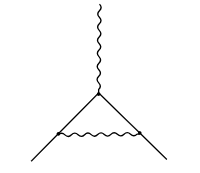
\includegraphics[width=0.2\linewidth]{img/1.png}
			\caption{Diagram contributing to QED vertex correction.}
			\label{ammdiag}
		\end{figure}

	
		\end{problem}
	\item
	\begin{problem}{\points{-}}
		\textbf{Dimensional Regularization:}
		The goal of this problem is to work out the following integral:
		\[
		\int \frac{d^dk}{(2\pi)^4} \frac{k^2a}{(k^2 - \Delta)^b}
		\].
		If we have such a powerful result at our disposal, we only need to use Feynman parametrization to complete-square the denominator and use this formula.
		
		The dimensional regularization scheme, as its name suggests, treats the dimension of the spacetime as a parameter to render finite amplitudes. In the end, we extract the divergent term by a limiting process. 
		
		Working out this integral also requires knowledge about $\beta-$function.
		\begin{enumerate}
			\item Take $\beta(a,b) = \int_0^1 dx x^{a-1} (1-x)^{b-1}$ as the definition of beta function. Do two change of variables to show that it is equal to:
			\begin{enumerate}
				\item $\frac{\Gamma(a)\Gamma(b)}{\Gamma(a+b)}$.
				\item $\int_0^\infty ds \frac{s^{a-1}}{(s+1)^{a+b}}$.(In this case take $x= \frac{s}{s+1}$.)
			\end{enumerate}
		\item In the original integral, rewrite the measure in spherical coordinates and do a Wick rotation, as you did in part (a).
		\item  Now compute the $\int dk_E \frac{k_E^{2a}}{(k^2_E +\Delta)^b}$ by using identities of the beta function.
		\item Put all things together to find:
		\begin{equation}
			\int \frac{d^dk}{(2\pi)^4} \frac{k^2a}{(k^2 - \Delta)^b} = i (-1)^{a-b} \frac{1}{(4\pi)^{\frac{d}{2}}} \frac{1}{\Delta^{b-a-\frac{d}{2}}}\frac{
			\Gamma(a+\frac{d}{2})	\Gamma(b-a-\frac{d}{2})
		}{\Gamma(b) \Gamma(\frac{d}{2})}
		\label{mainint}
		\end{equation}
	
		Now, finding the divergent part of the amplitudes boils down to knowing the divergences of $\Gamma(z)$ function. For our purposes, only $\Gamma(\epsilon) = \frac{1}{\epsilon} -\gamma_E + \mathcal{O}(\epsilon)$ is enough\footnote{$\gamma_E$ is the Euler-Mascheroni constant which is about 0.577 .}.
		
		The regularization procedure is to take $d = 4-\epsilon$ in the \eqref{mainint}, and extract the divergent term by the expansion of the Gamma function around zero. As an example let's regularize $\int \frac{d^dk}{(2\pi)^4} \frac{1}{(k^2-\Delta+i\epsilon)^2}$, which is equal to 
		$\frac{i}{(4\pi)^{\frac{d}{2}}} 
		\frac{1}{\Delta^{2-\frac{d}{2}}}\Gamma(\frac{4-d}{2}).
		$
		Expanding $d= 4 - \epsilon$ give the following result:
		\[
		\frac{i}{16\pi^2} (\frac{4\pi}{\Delta})^{\frac{\epsilon}{2}}(\frac{2}{\epsilon} - \gamma_E + \mathcal{O}(\epsilon))
		\]
		Remember that $a^\epsilon = e^{\epsilon \ln(a)} = 1+\epsilon \ln(a)$, as $\epsilon \to 0$, hence we get:
		\[
		\frac{i}{16\pi^2}\frac{1}{\epsilon} + 	\frac{i}{16\pi^2}\ln(\frac{4\pi e^{-\gamma_E}}{\Delta}) + \mathcal{O}(\epsilon)
		\] as our divergent and convergent parts respectively, and the $\epsilon$-dependent parts vanish in the limit.
		\end{enumerate}
	\textbf{Aside:} Some useful identities  that we encounter frequently are:
	\[
	\int\frac{d^dk}{(2\pi)^4} \frac{1}{(k^2-\Delta+i\epsilon)^2} = \frac{i}{(4\pi)^{\frac{d}{2}}}\frac{1}{\Delta^{2-\frac{d}{2}}}\Gamma(\frac{4-d}{2})
	\]
		\[
	\int\frac{d^dk}{(2\pi)^4} \frac{k^2}{(k^2-\Delta+i\epsilon)^2} = -\frac{d}{2}\frac{i}{(4\pi)^{\frac{d}{2}}}\frac{1}{\Delta^{1-\frac{d}{2}}}\Gamma(\frac{2-d}{2})
	\]
			\[
	\int\frac{d^dk}{(2\pi)^4} \frac{k^2}{(k^2-\Delta+i\epsilon)^3} = \frac{d}{4}\frac{i}{(4\pi)^{\frac{d}{2}}}\frac{1}{\Delta^{2-\frac{d}{2}}}\Gamma(\frac{4-d}{2})
	\]
	\end{problem}

	\item
\begin{problem}{\points{-}}
	\textbf{Dimensional Regularization Subtlties:}

	Since we change the dimension of the spacetime, so the dimension of the fields and the couplings in the problem should also change.
	\begin{enumerate}
		\item In QED Lagrangian, find the mass dimension of $A_\mu, \Psi, m, e$ in d-dimensional spacetime.
		\item To make coupling constant $e$ dimensionless, show that we have to change $e \to \mu^{\frac{4-d}{2}} e$, where $\mu$ is an arbitrary scale (not infinite!). We should justify later that the observables are independent of this scale\footnote{The dependence of regularized amplitude to this scale is like
	$\ln(\frac{4\pi e^{-\gamma_E}\mu^2}{\Delta})$.
	}.
	\end{enumerate}
\end{problem}

\end{enumerate}

\newpage
	\section*{Problem 2: Vacuum Polarization Diagram}

\begin{problem}
	Vacuum polarization involves a process in the vacuum of the theory where a pair of charged particles (e.g. $e^-e^+$ particles in QED)is created and annihilated  immediately. This virtual dipole is of significant importance in observations. Here, we work out the QED vacuum polarization diagram compeletely.
	\end{problem}

\begin{enumerate}
	\item
	\begin{problem}{\points{-}}
		\textbf{The amplitude:}
		
		Write down the amplitude of the vacuum polarization diagram according to QED‌ Feynman rules in momentum space. (The figure \ref{vaccpoldiag} shows the Feynman diagram.)
		\begin{figure}[H]
			\centering
			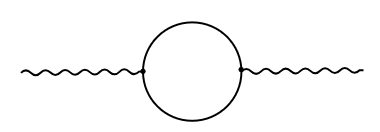
\includegraphics[width=0.35\linewidth]{img/2.png}
			\caption{Vacuum Polarization diagram in QED.}
			\label{vaccpoldiag}
		\end{figure}

	\end{problem}
\item
\begin{problem}{\points{-}}
	\textbf{Trace Technology:}
	
	To simplify the numerator, use these two identities in Clifford algebra:
	$Tr(\gamma^\mu\gamma^\nu) = 4\eta^{\mu\nu}$,
	$Tr(\gamma^\alpha\gamma^\mu\gamma^\beta\gamma^\nu) = 4\big(
	\eta^{\alpha\mu}\eta^{\beta\nu}-\eta^{\alpha\beta}\eta^{\mu\nu}+\eta^{\alpha\nu}\eta^{\beta\mu}
	\big)$. You should end up to:
	\[
	Tr\big[
	\gamma^\mu (\slashed{k}-\slashed{p}+m)\gamma^\nu (\slashed{k}+m)
	\big]=
	4\big[
	-p^\mu k^\nu - k^\mu p^\nu + 2k^\mu k^\nu + \eta^{\mu\nu} (-k^2 +p.k+m^2)
	\big]
	\]
	
\end{problem}
\item
\begin{problem}{\points{-}}
	\textbf{Drop Unnecessary Terms:}
	
	Now justify you can drop the $p^\mu k^\nu$ part of the integral, use odd integrand argument to conclude these terms vanish after integration.
	
\end{problem}
\item
\begin{problem}{\points{-}}
	\textbf{Feynman Trick:}
	
	Introduce Feynman parametrization to complete square the denominator, then change the variables of integration according to $k^\mu \to k^\mu + p^\mu (1-x)$. Show that the Jacobian is unit.
	
	You have to have something like this:
	\[
	\Pi^{\mu\nu}_2 = 4ie^2 \int_0^1 dx\int \frac{d^dk}{(2\pi)^4} 
	\frac{
2k^\mu k^\nu - \eta^{\mu\nu}(k^2 -x(1-x) p^2 -m^2)	
}{(k^2 +p^2x(1-x) -m^2)^2}
	\]
	
\end{problem}
\item
\begin{problem}{\points{-}}
	\textbf{Dimensional Regularization:}
	
	Use D.R. to regularize this amplitude. There's another trick that you should utilize: replace $k^\mu k^\nu$ by $\frac{1}{d} \eta^{\mu\nu}k^2$. \footnote{Can you justify this innocent trick?}
	
	\[
	\Pi^{\mu\nu}_2 = -\frac{e^2}{2\pi^2}p^2\eta^{\mu\nu}\Big(
	\int_0^1 dx \; x(1-x) \Big[
	\frac{2}{\varepsilon} \ln \big(\frac{\tilde{\mu}^2}{m^2 - p^2x(1-x)}\big) +\mathcal{O}(\varepsilon)
	\Big]
	\Big)
	\]
	
\end{problem}

\item
\begin{problem}{\points{-}}
	\textbf{Reviving Gauge Invariance:}
	
	As we've promised, D.R. should preserve gauge invariance (or Ward Identity.) But this is not manifest in the regularized amplitude in part (e). The idea is that we hadn't considered the full amplitude yet, which consists of $p^\mu p^\nu$ terms.
	
	Do so and end up with\footnote{I know it's tedious, but absolutely necessary!}:
	\[
	\Pi^{\mu\nu}_2 = -\frac{8e^2}{(4\pi)^{\frac{d}{2}}} (p^2 \eta^{\mu\nu} - p^\mu p^\nu) \Gamma(2-\frac{d}{2}) \mu^{4-d} \int_0^1 dx (1-x)x \big(\frac{1}{m^2 - p^2x(1-x)}\big)^{2-\frac{d}{2}}
	\]
	So we recover the gauge invariance in the one-loop level.
\end{problem}
\end{enumerate}

\newpage
	\section*{Problem 3: Physics of the Vacuum Polarization}
	As we saw,
	\[
	i\Pi^{\mu\nu}_2 = -i (p^2 \eta^{\mu\nu} - p^\mu p^\nu) e^2 \Pi_2(p^2),
	\]
	Where
	\[
	\Pi_2(p^2) = \frac{1}{2\pi^2} \int_0^1 dx(1-x)x \big(\frac{2}{\epsilon} + \ln(\frac{\tilde{\mu}^2}{m^2-p^2x(1-x)})\big).
 	\]
	
\begin{enumerate}
	\item
	\begin{problem}{\points{-}}
		\textbf{The Dressed Propagator $G^{\mu\nu}$:} 
		
		Dressed Propagator could be interpreted as Fourier transform of the corrected Coloumb potential, i.e.
		\begin{figure}[H]
			\centering
			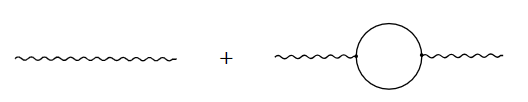
\includegraphics[width=0.6\linewidth]{img/3.png}
			\caption{The dressed propagator up to one-loop level.}
			\label{dressprop}
		\end{figure}
	Conclude that $iG^{\mu\nu} = -\frac{i}{p^2} (1-e^2\Pi_2(p^2))\eta^{\mu\nu}$.
	\end{problem}

	\item
	\begin{problem}{\points{-}}
		\textbf{Renormalization condition:} 
		
		Now it's time to define a renormalization condition. It's pretty natural to expect that all the quantum effects are in electric charge and the Coloumb potential (in momentum space) is the same as before, with $e_R$ instead of bare $e$.
		\[
		\tilde{V}(p_0^2) = \frac{e^2_R}{p^2_0}
		\]
		
		Now solve $e_R$ in terms of $e$, then find renormalized potential, which is:
		\[
		\tilde{V}_R(p^2) = \frac{e^2_R}{p^2}\Big(
		1+ \frac{e^2_R}{2\pi^2} \int_0^1 dx (1-x)x\ln(1-\frac{p^2}{m^2}x(1-x))+ \mathcal{O}(e^4_R)
		\Big)
		\]
	\end{problem}
\textbf{Aside:} The renormalized potential reproduces the Lamb shift in the limit $m^2 \gg |p^2|$(or Hydrogen atom in low-energy.) The process involves calculating integral with this approximation and then do an inverse Fourier transformation to see Dirac delta function in the position space\footnote{
For more detail, consult to 16.3.1 Schwartz}.
\end{enumerate}






\end{document}